\begin{savequote}[75mm]
Basic research is what I am doing when I don't know what I am doing.
\qauthor{Wernher von Braun}
\end{savequote}

\chapter{$H\rightarrow WW^{*}\rightarrow \ell\nu\ell\nu$ Analysis Strategy}

\section{Introduction}

This chapter will present an overview of the strategy for searching for a Higgs boson in the 
\HWWfull decay topology. Its purpose is to present in broad terms how the search and measurement are undertaken, before going into details on the specific sub-categories within the broader analysis. 

First, the topology of the signal final state and corresponding backgrounds are
presented. Next, an overview of the variables used to reduce the backgrounds and enhance the
signal is given. These will be described in general, while specific values of selection cuts and background estimation will be provided in subsequent chapters. Finally, the parameters of interest in the search and measurement will be defined, 
and a brief overview of the statistical treatment of the final Higgs candidates is shown.


\section{Signal topology}

\label{sec:sigtopology}

The analysis presented here and in subsequent chapters is the study of the Higgs boson in the $WW$ final state,
where each $W$ boson subsequently decays into a charged lepton and a neutrino. In its simplest form, the final state will then consist of two neutrinos and two charged leptons, each of which can be either an electron or a muon. If one or both of the $W$s decay to $\tau$ leptons, only leptonic decays of the $\tau$ are considered, leading to additional neutrinos in the final state but still giving two charged leptons as before. Neutrinos are not detected in ATLAS, so the final state ultimately consists of two reconstructed leptons and \met (denoted as $\MET$). Final states where both of the charged leptons are electrons or muons are referred to as the ``same flavor" final states, while those with one electron and one muon are referred to as ``different flavor".

\begin{figure}
  \vspace{20pt}
  \centering
  \hspace*{-32pt}
  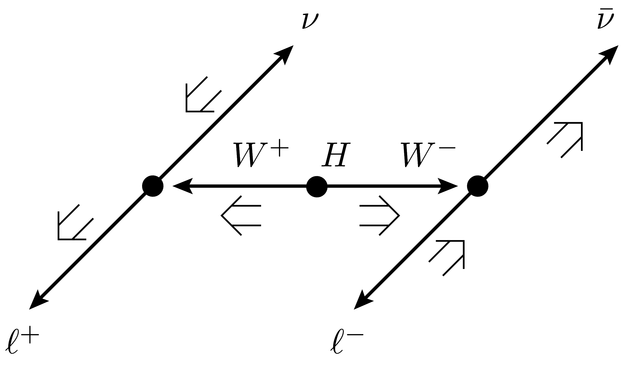
\includegraphics[width=0.42\textwidth]{figures/ww_spins}
  \caption{A cartoon of the WW final state. Momenta are represented with thin arrows, spins with thick arrows. \cite{WW2015}}
  \label{fig:HWWdiagram}
\end{figure}


The final state leptons will also exhibit unique correlations due to the fact that they are arising from the decay of a spin zero resonance. In particular, the spins of the final state leptons and neutrinos must all cancel, as shown in figure~\ref{fig:HWWdiagram}. Because the neutrino has a left handed
helicity and the anti-neutrino has a right handed helicity, the spin and momentum of the particles will be anti-aligned and aligned, respectively. In the transverse plane, the momenta of all four final state objects must cancel as well. With the constraint of having both the momenta and the spin alignments cancel, the final state kinematics strongly prefer having a small angle between the leptons in the transverse plane (low $\dphill$). This angular correlation will also lead to low values of the di-lepton invariant mass $\mll$. These unique signal final state kinematic correlations will be exploited to define the ultimate signal region. 

While the basic final state consists of two leptons and $\MET$, there can be additional objects as well depending on the production mode of the Higgs. As described in detail in Chapter 1, if the Higgs is produced via vector boson fusion production, there will be two additional forward jets in the event. Even in gluon fusion, one or more jets can be produced through initial state radiation from the incoming gluons. The analysis is separated into different signal regions depending on the number of hard jets reconstructed in the final state as well.


\section{Background processes}

Many processes from the Standard Model can also produce a final state with two leptons and \met. This section lists the dominant backgrounds to Higgs production. It gives general descriptions of how the backgrounds mimic Higgs production and how they can be reduced. The details of background estimation and specific cuts are left for later sections. Table\ref{tab:bkgtable} summarizes the different processes. 

\subsection{Standard Model WW production}

\begin{figure}[h!]
  %\vspace{20pt}
  \centering
  \captionsetup{justification=centering}

  %\hspace*{-32pt}
  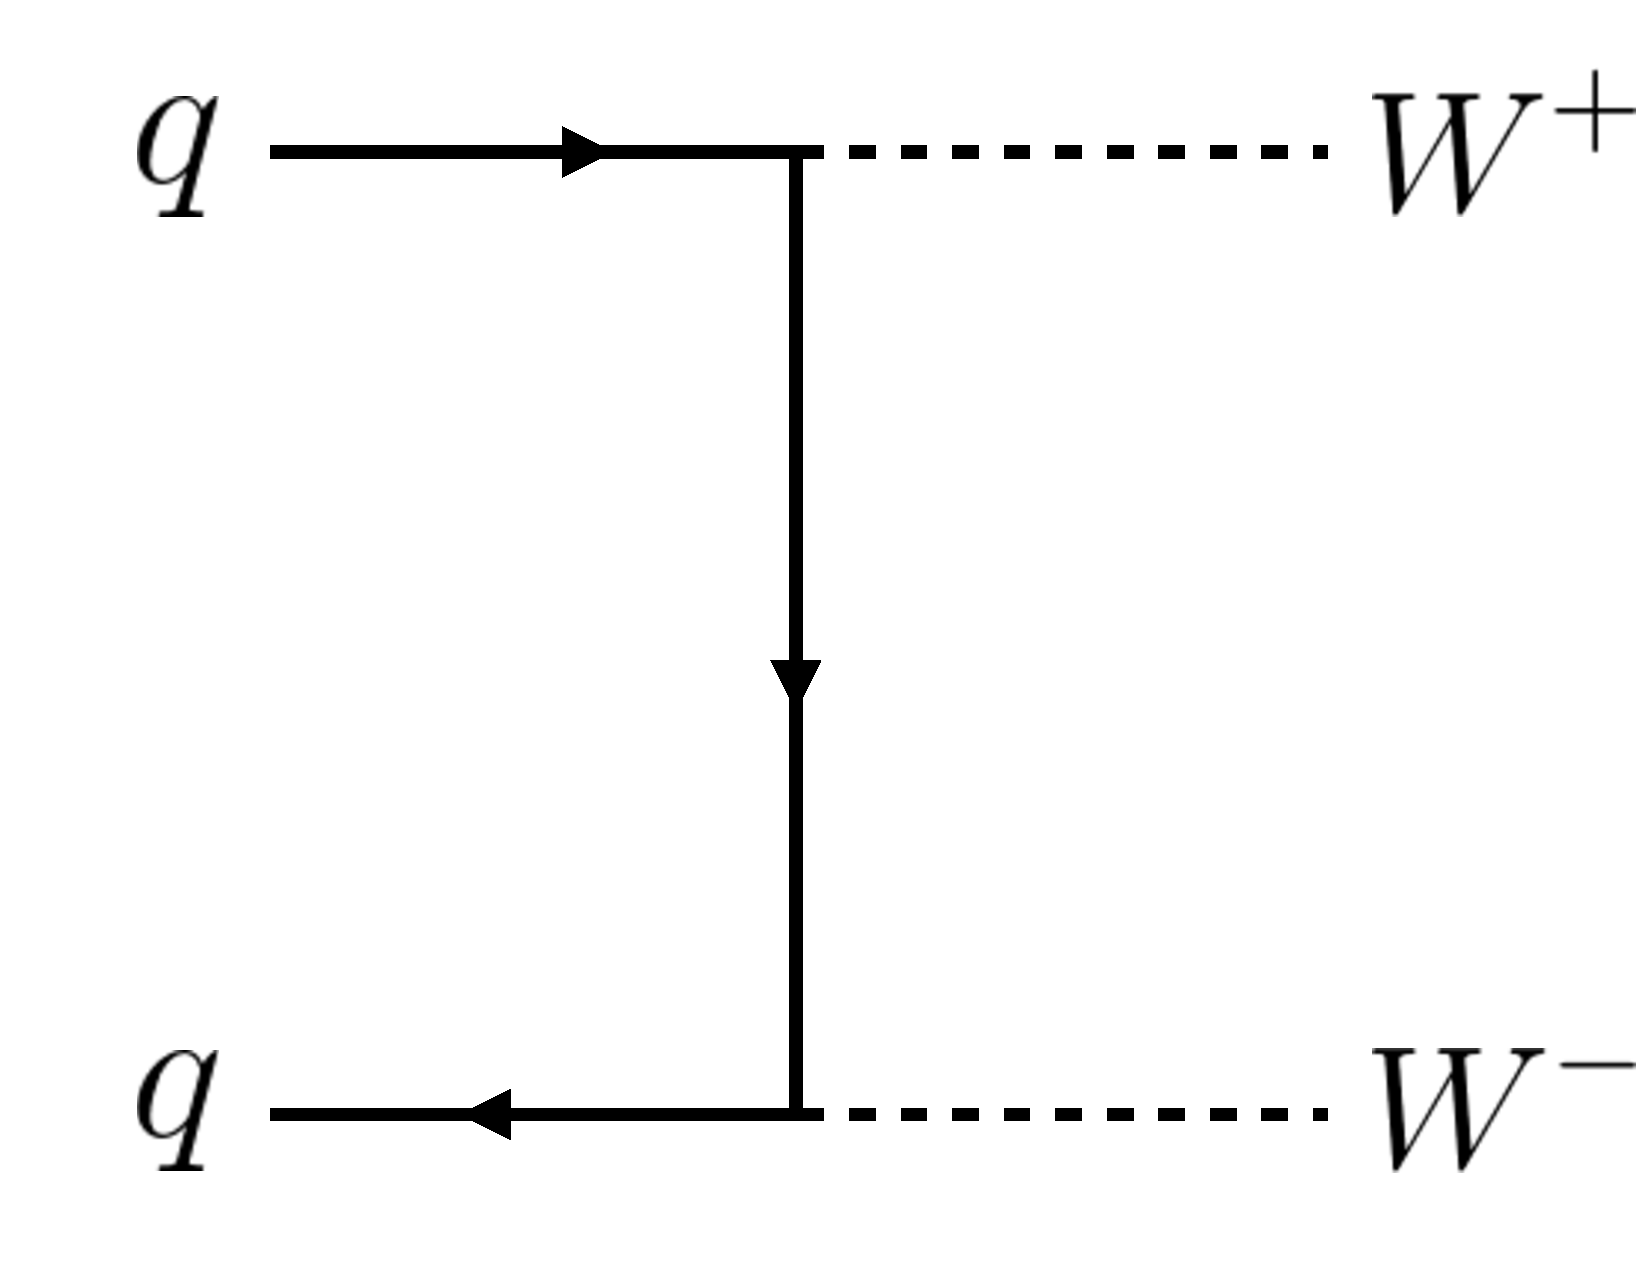
\includegraphics[width=0.2\textwidth]{figures/Feyn_SMWW}
  \caption{Feynman diagram for Standard Model WW production}
  \label{fig:SMWWdiagram}
\end{figure}

Non-resonant Standard Model diboson production, as shown in figure~\ref{fig:SMWWdiagram}, is an irreducible background to Higgs boson production in the WW final state. It produces the same exact final state objects, namely leptonically decaying W bosons. There are no additional objects in the final state that allow for background reduction. Therefore the analysis solely relies on the correlations between the leptons to reduce this background. 

\subsection{Top quark production}

Production of top quarks, either in pairs ($\ttbar$ production) or singly (e.g. $Wt$ production), can also mimic Higgs production. Because top quarks decay via $t\TO Wb$, top pair production can  produce a final state with two W bosons that then decay leptonically. In this case, however, there are two additional jets from the bottom quarks in the final state. This allows the analysis to veto on the presence of jets identified as originating from a $b$ in order to reduce the size of the background. 

Single top production can occur via $s$-channel, $t$-channel, or associated production ($Wt$). The mode which most closely resembles the Higgs final state is $Wt$. In this case, there are two real $W$ bosons produced, as with $\ttbar$. However, the decay of the single top quark will still also produce one $b$-jet, meaning a $b$ veto will reduce this background as well. 

Figure~\ref{fig:Topdiagram} shows the Feynman diagrams for $\ttbar$ and $Wt$ production.  

\begin{figure}[h!]
  %\vspace{20pt}
  \centering
  \captionsetup{justification=centering}

  %\hspace*{-32pt}
  \raisebox{-0.5\height}{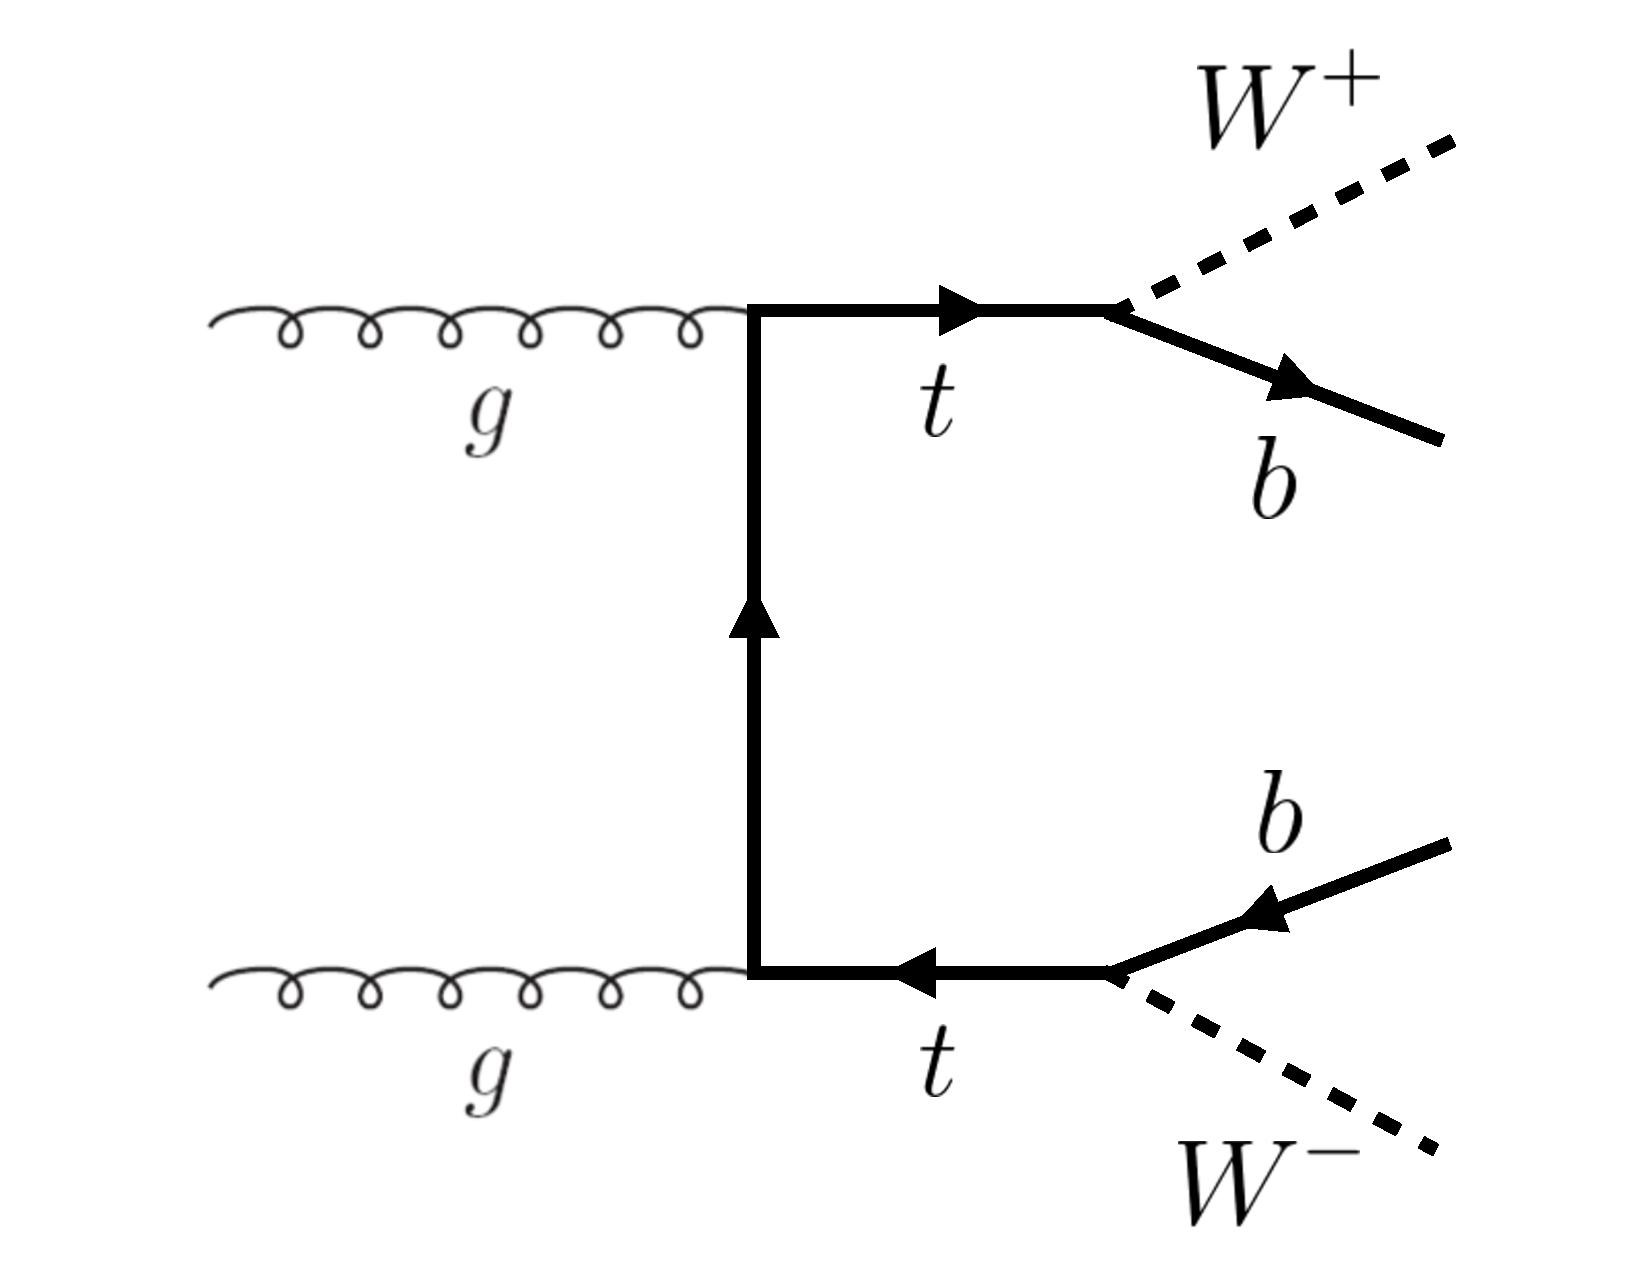
\includegraphics[width=0.2\textwidth]{figures/Feyn_ttbar}}
  \hspace{20pt}
  \raisebox{-0.5\height}{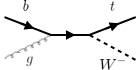
\includegraphics[width=0.2\textwidth]{figures/Feyn_Wt}}
  \caption{Feynman diagrams for top pair production (left) and $Wt$ production (right)}
  \label{fig:Topdiagram}
\end{figure}

\subsection{$W$+jets background}

Single $W$ boson production, in association with jets, is a unique background. The other background considered so far have all included real leptons in the final state. In this case, however, only one real lepton from the decay of a $W$ exists in the final state. The second reconstructed lepton can arise from two different cases. First, the lepton may truly be an algorithm ``fake", or a jet misidentified as a lepton by either the electron or muon reconstruction algorithms. Second, the lepton may be a real lepton but coming from semi-leptonic decays of particles inside the shower of the jet. This background can be reduced by requiring that the reconstructed lepton have little activity surrounding it in the calorimeter (also known as an ``isolated" lepton). Figure~\ref{fig:Wdiagram} shows the Feynman diagram for $W$+jets production. 


\begin{figure}[h!]
  %\vspace{20pt}
  \centering
  \captionsetup{justification=centering}

  %\hspace*{-32pt}
  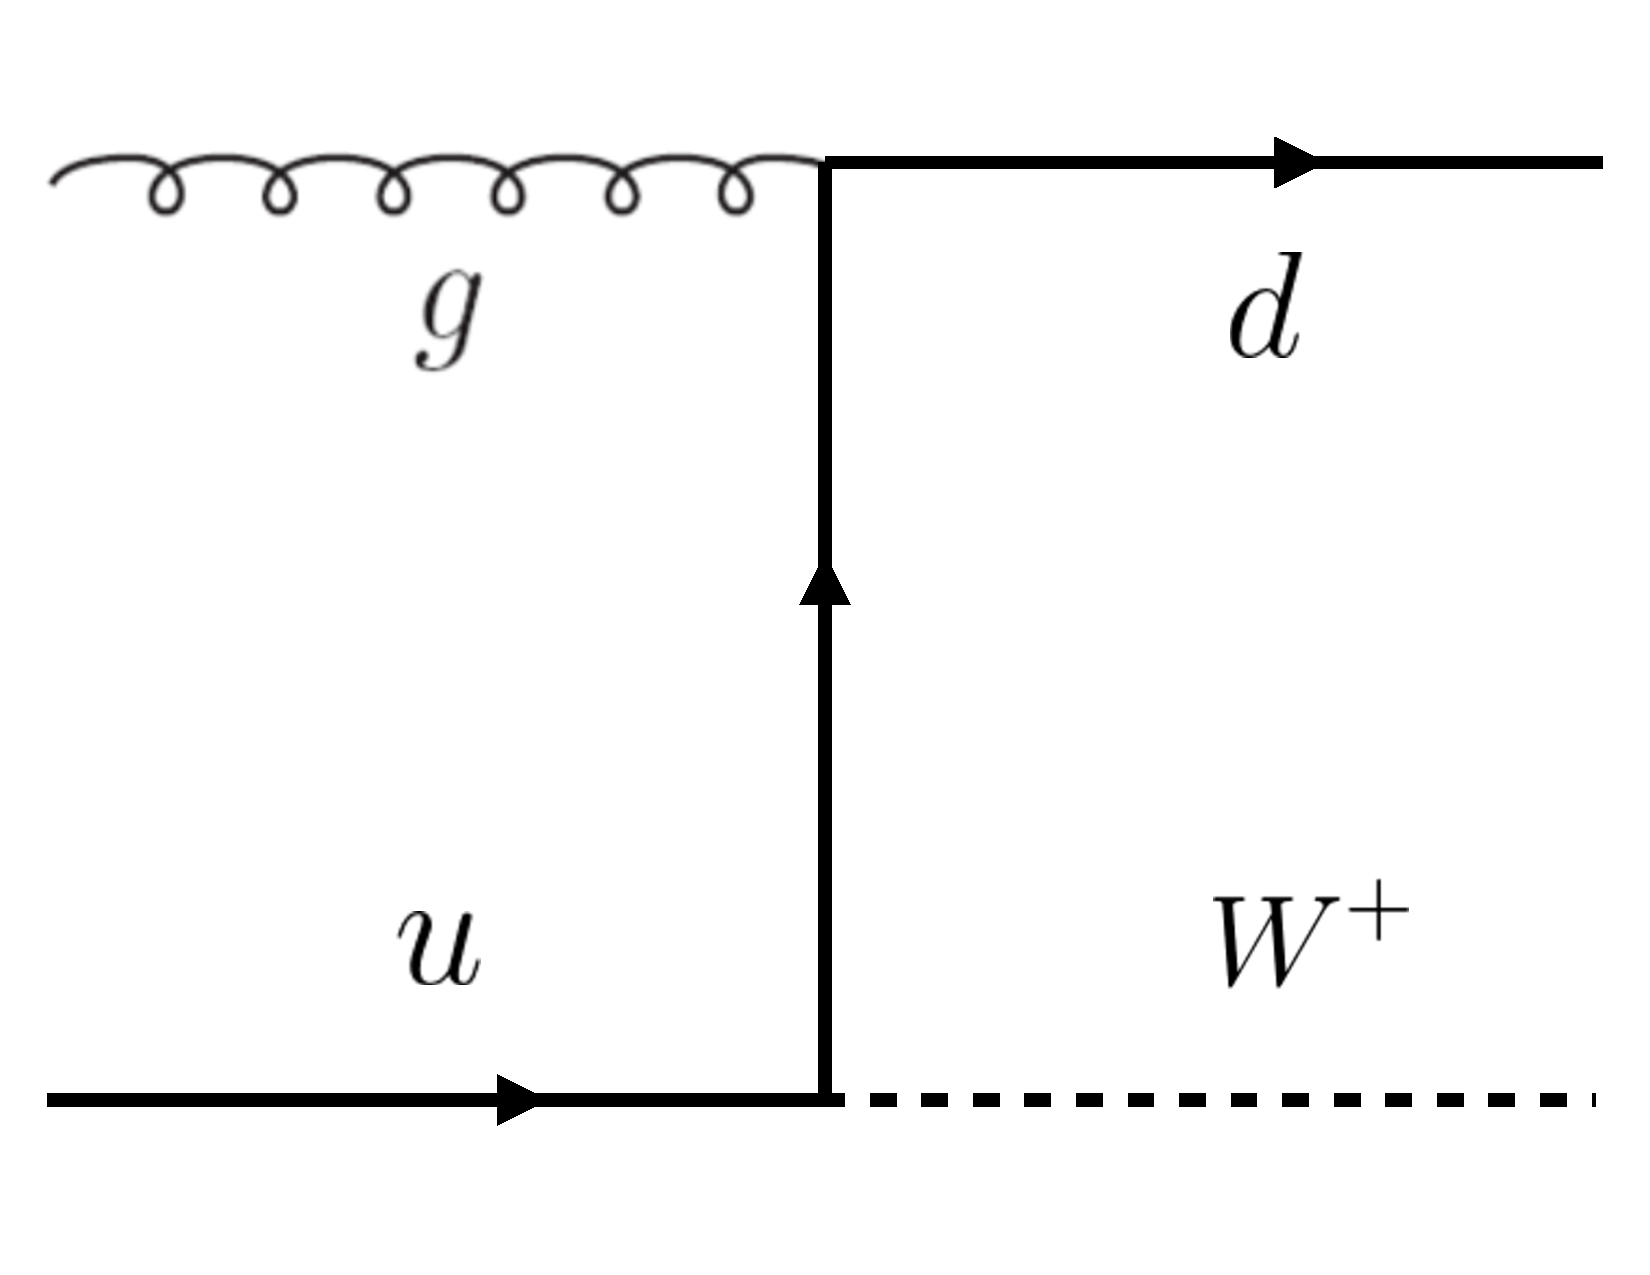
\includegraphics[width=0.2\textwidth]{figures/Feyn_W}
  \caption{An example Feynman diagram of $W$+jets production}
  \label{fig:Wdiagram}
\end{figure}

\subsection{$Z/\gamma^{*}$+jets background}

Production of a $Z/\gamma^{*}$  in association with jets (also known as Drell-Yan) is also a background to Higgs production. In particular, the same flavor final states have a large $Z$+jets background, as the $Z$ decays into two leptons of the same flavor. (This background also enters the different flavor final state through the leptonic decays of $Z\TO\tau\tau$). Figure~\ref{fig:Zdiagram} shows the production of a $Z$ in association with one jet. Because there are no neutrinos in this final state, variables like $\MET$ can be used to reduce the background. 

\begin{figure}[h!]
  %\vspace{20pt}
  \centering
  \captionsetup{justification=centering}

  %\hspace*{-32pt}
  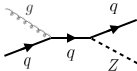
\includegraphics[width=0.2\textwidth]{figures/Feyn_Zjets}
  \caption{An example Feynman diagram of $Z$+jets production}
  \label{fig:Zdiagram}
\end{figure}

\subsection{Other (subdominant) backgrounds}

THere are additional processes which contrinute to the background composition but are not produced as frequently as those listed already. The first of these are referred to as $VV$ or ``Other diboson" processes and include multiple Standard Model diboson processes, including $WZ$, $ZZ$, $W\gamma$, $W\gamma^{*}$, and $Z\gamma$ production. Additionally, there is background from QCD multijet production, where two jets are misidentified as leptons. 

\begin{table}[h!]
\centering
\captionsetup{justification=centering}

%\begin{tabular*}{0.480\textwidth}{p{0.075\textwidth} p{0.180\textwidth} l}
\hspace{-10pt}
{\renewcommand{\arraystretch}{1.15}
\begin{tabular}{|c|c|c|}
\hline
Category & Process & Description \\ \hline
SM $WW$ & $WW\TO\ell\nu\ell\nu$ & Real leptons and neutrinos \\ \hline
\multirow{3}{*}{Top quark production} & $t\bar{t}\TO WbW\bar{b}\TO\ell\nu b \ell\nu \bar{b}$ & Real leptons, untagged $b$s \\ 
 & $tW \TO WbW \TO \ell\nu\ell\nu b $ & Real leptons, untagged $b$ \\ 
 & $t\bar{b}$, $tq\bar{b}$ & Untagged $b$, jet misidentified as lepton \\ \hline

 \multirow{2}{*}{Drell-Yan} & $\ZDY\TO ee, \mu\mu$ & ``Fake" $\MET$ \\ 
  & $\ZDY\TO \tau\tau \TO \ell\nu\nu \ell\nu\nu $& Real leptons and neutrinos \\ \hline

  \multirow{3}{*}{Other dibosons} & $ZZ \to \ell\ell \nu\nu$ & Real leptons and neutrinos \\ 
   & $W\gamma^{*}, WZ \TO \ell\nu\ell\ell, ZZ \to \ell\ell\ell\ell$ & Unreconstructed leptons \\ 
   & $W\gamma, Z\gamma$ & $\gamma$ reconstructed as $e$, unreconstructed lepton \\ \hline

   $W$+jets & $Wj \TO \ell\nu j$ & Jet reconstructed as lepton \\ \hline
   QCD multijet & $jj$ & Jets reconstructed as leptons \\ \hline
 
 \hline
\end{tabular}
}
%\end{tabular*}
\caption{
  A summary of backgrounds to the \HWWfull signal 
}
\label{tab:bkgtable}
\end{table}


%\section{Object definitions}

%Selecting objects for the analysis is the first step towards rejecting background while maintaining signal acceptance. Details of the object reconstruction algorithms are defined in Chapter 2. This section presents the selections applied for reconstructed electrons, muons, jets, and \met in the final Run 1 \HWWfull analysis in order to 


\section{Isolating an $H\rightarrow WW^{*}\rightarrow \ell\nu\ell\nu$ signal}

As presented in section~\ref{sec:sigtopology}, there are many different combinations of objects that can define a \HWWfull final state. The multiplicity of jets and the flavor combinations of the leptons both lead to a combinatorically large number of potential signal regions. Additionally, signal regions can be optimized separately to be sensitive to the distinct production modes of the Higgs. Gluon fusion, vector boson fusion, and associated production of a Higgs all lead to unique final state topologies. Figure~\ref{fig:analysisregions} delineates the different signal regions used in the gluon fusion and vector boson fusion $\HWW$ analyses. While there are different optimizations possible in each signal region, there are also some commonly shared selections that will be described here.

\begin{figure}[h!]
  %\vspace{20pt}
  \centering
  \captionsetup{justification=centering}

  %\hspace*{-32pt}
  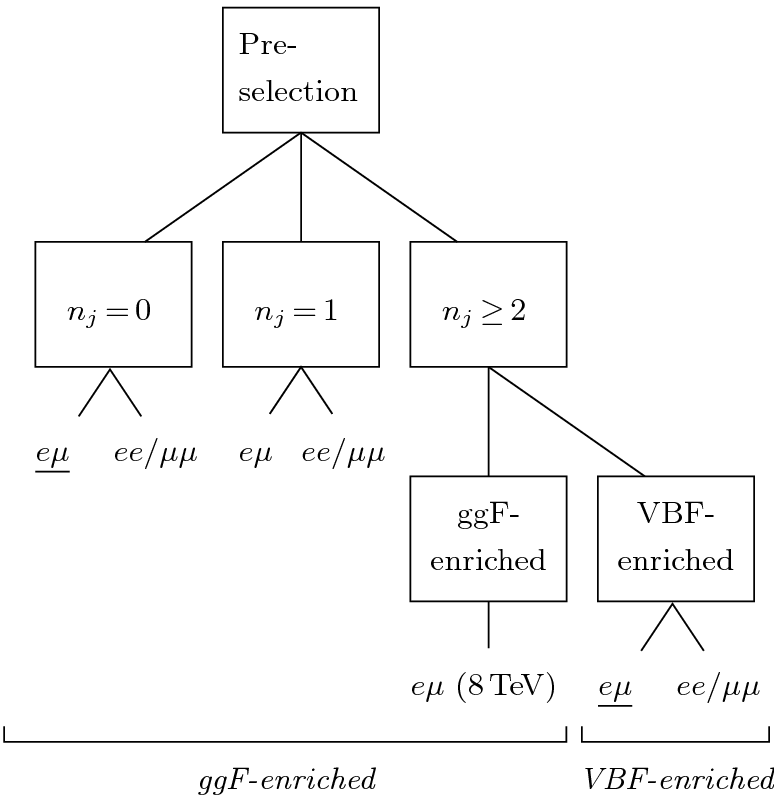
\includegraphics[width=0.6\textwidth]{figures/analysis_regions}
  \caption{An illustration of the unique analysis signal regions\cite{WW2015}}
  \label{fig:analysisregions}
\end{figure}

\subsection{Event pre-selection}

Before being sorted into the distinct signal regions, basic cuts are applied on the reconstructed objects in the event to select Higgs-like event candidates. First, two oppositely charged leptons are required. The $\pt$ threshold on the leptons is a particularly important consideration for this signal. Because the second $W$ produced in the decay can be off-shell, it tends to produce lower momentum leptons. Thus, being able to lower the $\pt$ threshold while still maintaining a low background rate is critical. Figure~\ref{fig:leptonpt} shows an example of the subleading lepton $\pt$ for a VBF $\HWW$ signal compared to the corresponding $t\bar{t}$ background. Note that the lepton $\pt$ spectrum is considerably softer in the signal sample. 

\begin{figure}[h!]
  %\vspace{20pt}
  \centering
  \captionsetup{justification=centering}

  %\hspace*{-32pt}
  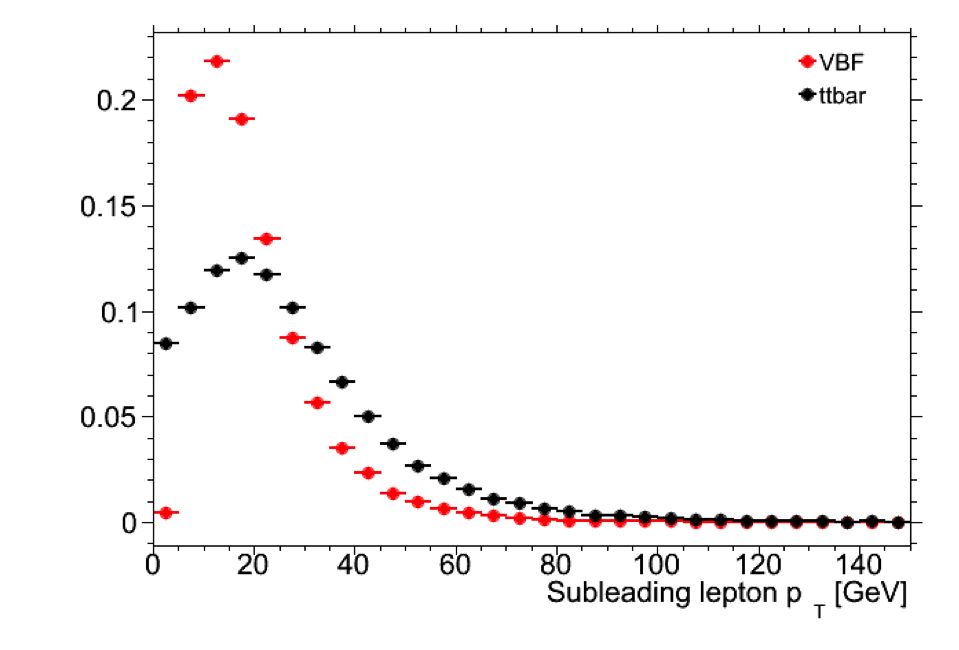
\includegraphics[width=0.6\textwidth]{figures/lepton_pt}
  \caption{A comparison of the subleading lepton $\pt$ spectrum between VBF $\HWW$ production and $t\bar{t}$ background}
  \label{fig:leptonpt}
\end{figure}

Once the leptons are selected, the last requirement for event pre-selection is the presence of neutrinos. As neutrinos cannot be detected directly in ATLAS, $\MET$ can be used as a proxy for the combined neutrino momentum in the transverse plane. In general, it is expected that the signal should have a harder $\MET$ spectrum than backgrounds, especially if those backgrounds did not contain neutrinos. One additional consideration when using $\MET$ is the fact that mis-measurements of objects in the detector can lead to imbalances in the transverse plane that are not due to real particles escaping the detector. One indicator that this is the case is that the $\MET$ vector in the transverse plane will be pointing in the same direction as the mis-measured object. Therefore, a new variable, $\METrel$, is used in the pre-selection. $\METrel$ is defined in equation~\ref{eqn:METrel}. 

\begin{equation}
  \begin{array}{ll}
  \multirow{2}{*}{$\METrel$ =\ \bigg\{ }
    &\!\!\!\!\MET\ \sin\dphiNear\quad\textrm{if $\dphiNear<\pi/2$}\\
    &\!\!\!\!\MET\ \phantom{\sin\dphiNear}\quad\textrm{otherwise,}
  \end{array}
\label{eqn:METrel}
\end{equation}

If the closest object to the $\MET$ vector is within $\pi/2$ radians in the transverse plane, the $\MET$ is projected away from this object. Otherwise, the normal $\MET$ vector is used. Figure~\ref{fig:METrel} shows a graphical illustration of this concept. 

\begin{figure}[h!]
  %\vspace{20pt}
  \centering
  \captionsetup{justification=centering}

  %\hspace*{-32pt}
  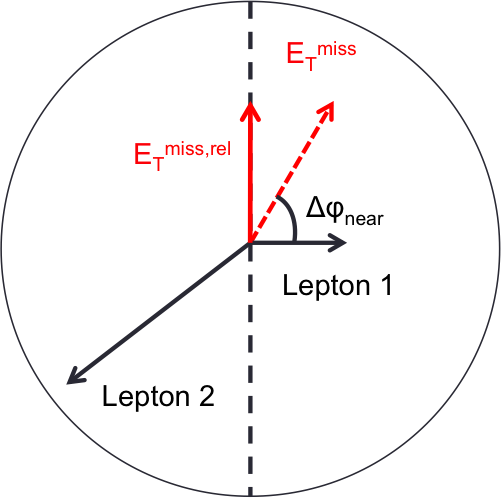
\includegraphics[width=0.6\textwidth]{figures/METrel_cartoon}
  \caption{A graphical illustration of the $\METrel$ calculation}
  \label{fig:METrel}
\end{figure}

Once both the lepton and $\MET$ pre-selections are made, the analysis can be divided into different regions according to jet multiplicity.

\subsection{Jet multiplicity}
\label{sec:jetmult}
Jet multiplicity, denoted as $\Njet$, is used to sub-divide the analysis into its distinct signal regions. The reason for this is twofold. First, different jet multiplicity bins will be more or less sensitive to different Higgs production modes. For example, the $\Njet \geq 2$ region is more sensitive to VBF production because of the two hard jets produced at matrix element level. For gluon fusion production to enter this bin, two initial state radiation jets must be emitted. Second, background composition varies greatly in different bins of $\Njet$. Figure~\ref{fig:njet} shows the jet multiplicity in both the different flavor and same flavor regions. It also shows the background composition in the bins of $\Nbjet$. There are a few clear trends from this distribution. The first is that the Drell-Yan background dominates in the same flavor channels for $\Njet \leq 1$. Second, the top background becomes a clear contributor to the total background for $\Njet \geq 1$. Lastly, the SM WW production dominates in the $\Njet = 0$ bin, as it is an irreducible background to $\HWW$ production. Because of these distinct features, each jet multiplicity bin is treated separately.

\begin{figure}[h!]
  %\vspace{20pt}
  \centering
  \captionsetup{justification=centering}

  %\hspace*{-32pt}
  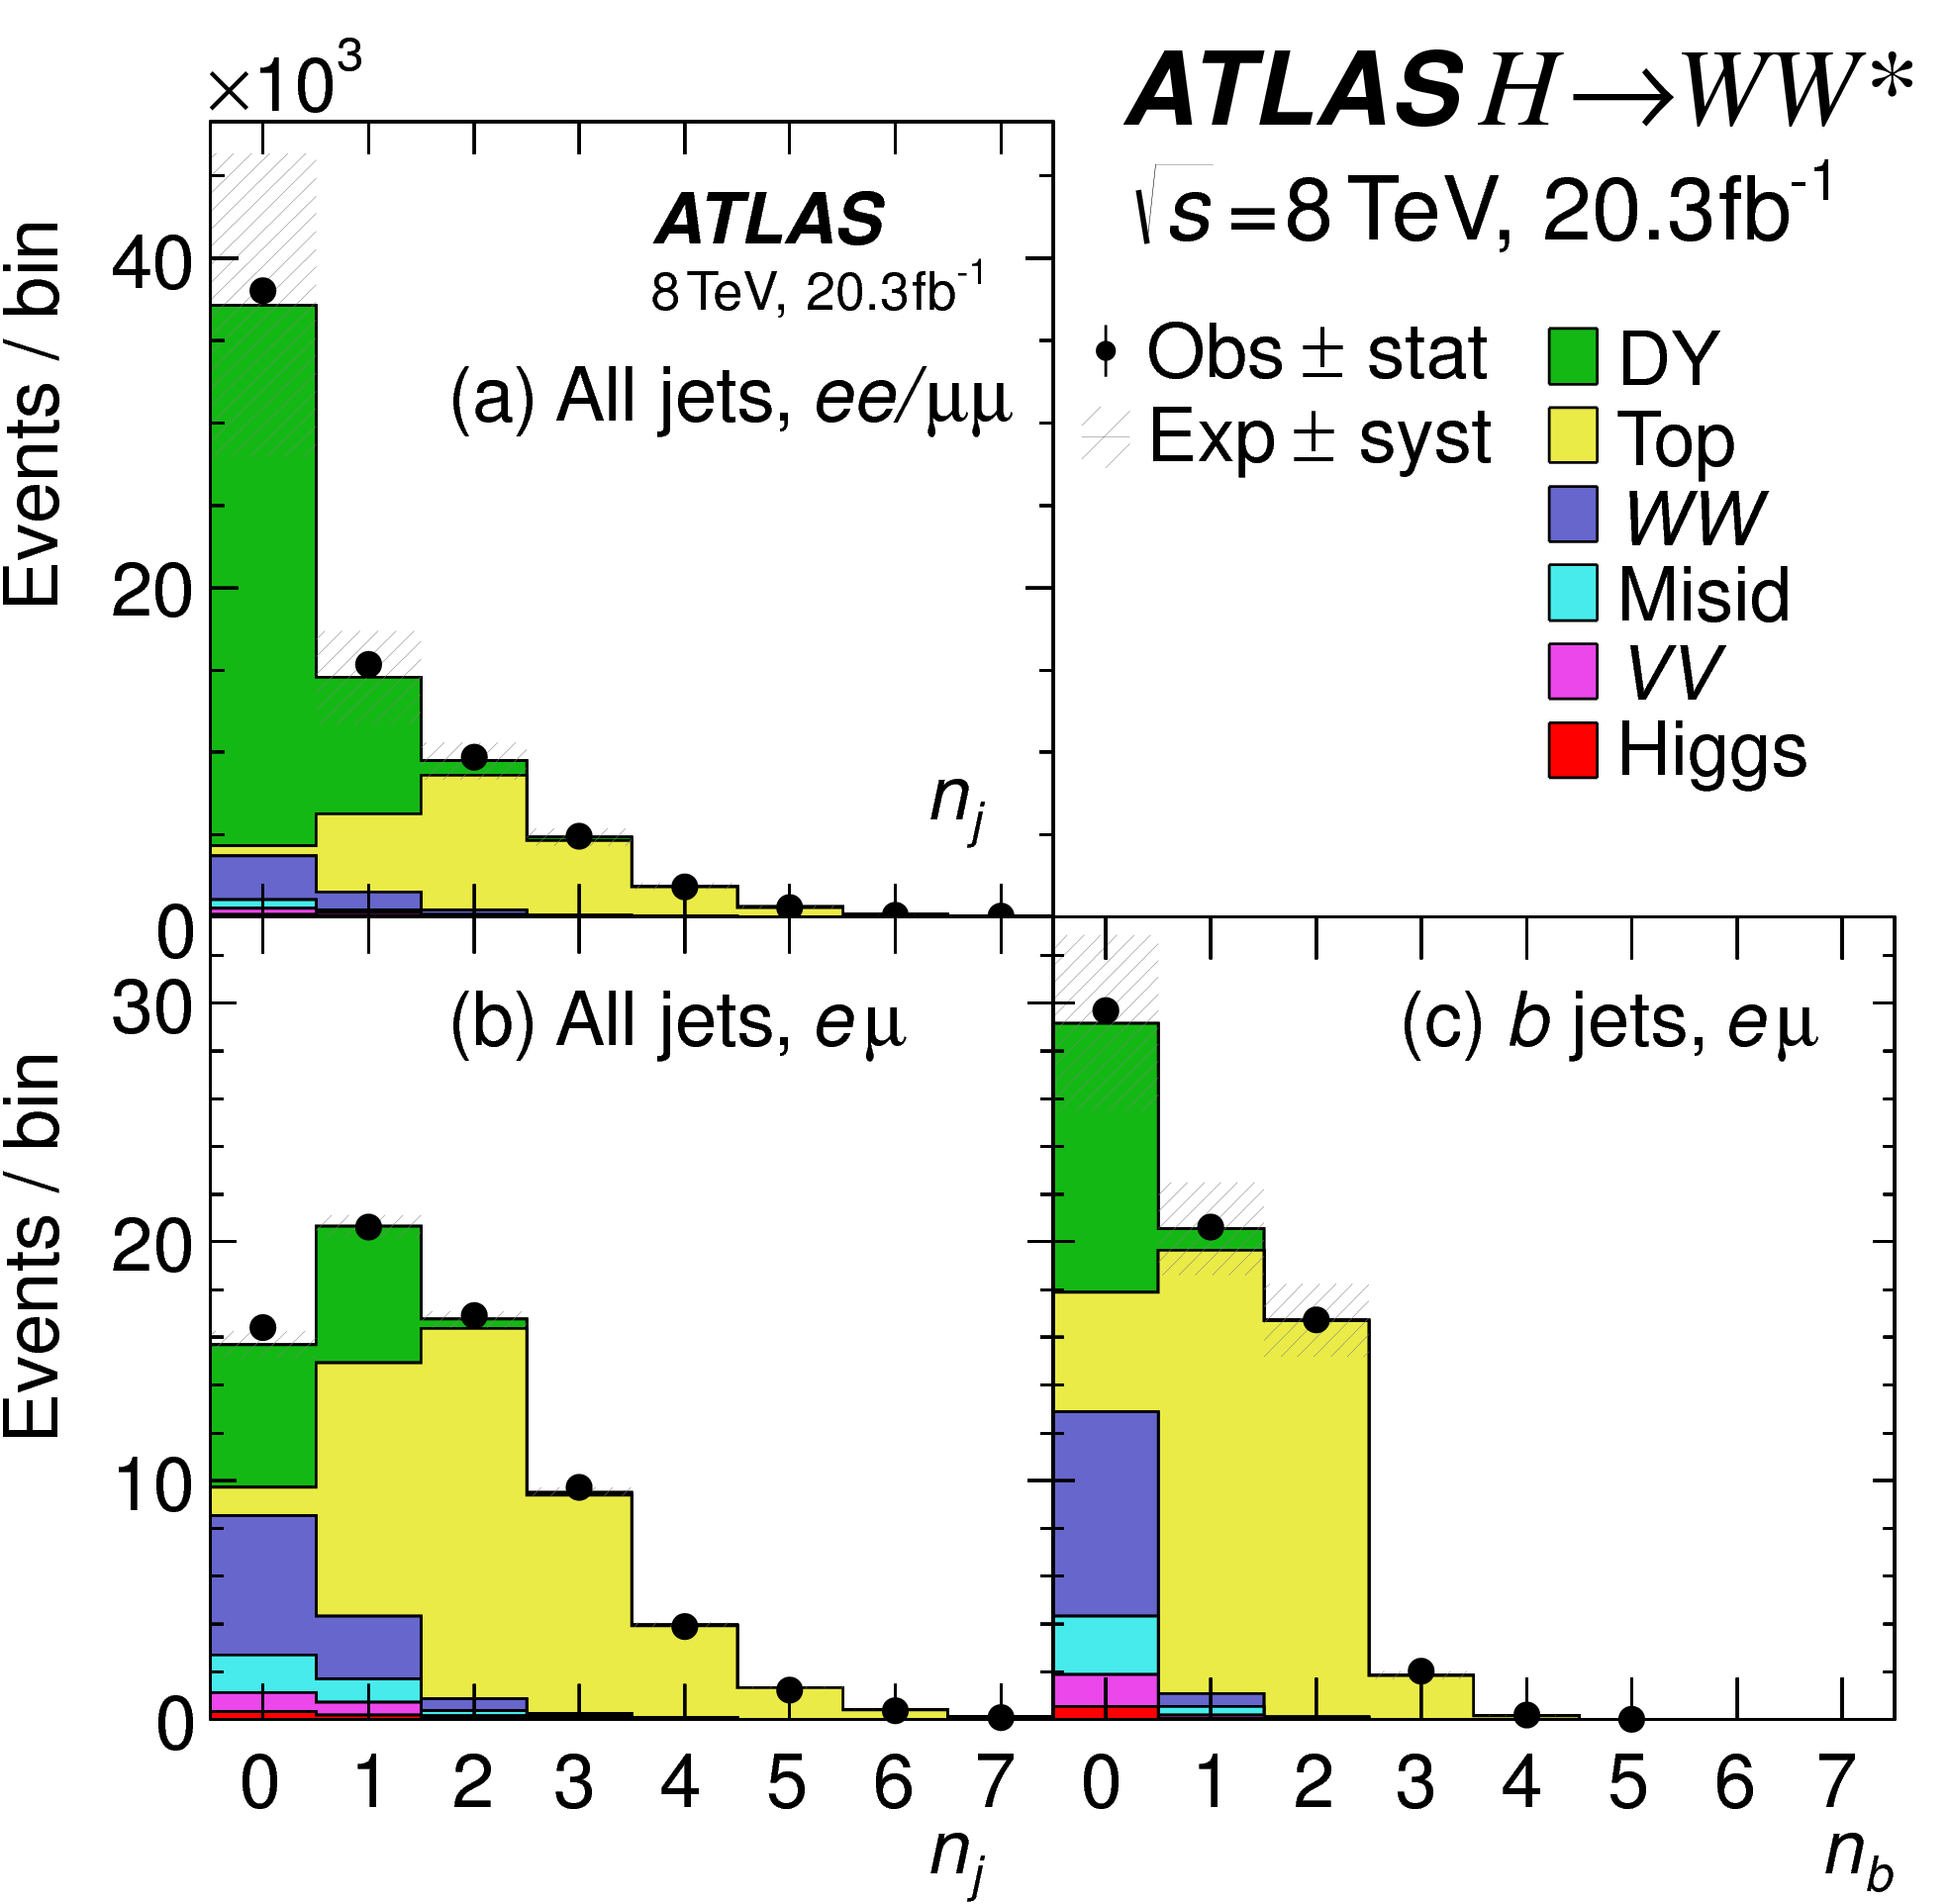
\includegraphics[width=0.6\textwidth]{figures/njet}
  \caption{Predicted backgrounds (compared with data) as a function of $\Njet$ (a and b) and $\Nbjet$ (c)}
  \label{fig:njet}
\end{figure}

\section{Background reduction in same-flavor final states}

As described in section~\ref{sec:jetmult}, the background composition of the same flavor final states is unique to that of the different flavor states. In particular, Drell Yan processes play a much larger role because the $Z/\gamma^{*}$ decays to same flavor leptons. Because real neutrinos are absent in the $\ZDY$ decays to $ee$ and $\mu\mu$, a cut on $\MET$ should largely reduce the background. However, as this section will demonstrate, with increasing pileup conditions the resolution of the calorimeter-based $\MET$ degrades greatly. Therefore, two new variables for $\ZDY$ background reduction are constructed and described in this section.

\subsection{Pileup and $\MET$ resolution}

Secondary interactions of protons in the colliding bunches of the LHC (known as pileup interactions, described in detail in Chapter 2) deposit energy into the ATLAS calorimeter on top of the energy that comes from the hard scatter process that is being searched for or analyzed. The calculation of $\MET$ is fundamentally Poissonian, as summing up all of the energy deposits in individual calorimeter cells or clusters is similar to a counting experiment. Thus, the energy resolution scales as $\sqrt{E}$, just as the error on a mean of $N$ in a Poisson distribution is $\sqrt{N}$. As more energy is deposited in the calorimter, the $\MET$ resolution degrades, meaning that the $\MET$ resolution is particularly sensitive to LHC instantaneous luminosity conditions. 

Figure~\ref{fig:Zjetseventdisplay} shows an event display of a $\ZDY$ + jets event candidate with the twenty-five reconstructed primary vertices. This display illustrates that while the interaction of interest only has tracks coming from the hardest primary vertex, all of the secondary interactions will deposit energy in the calorimeter as well.

\begin{figure}[h!]
  %\vspace{20pt}
  \centering
  \captionsetup{justification=centering}

  %\hspace*{-32pt}
  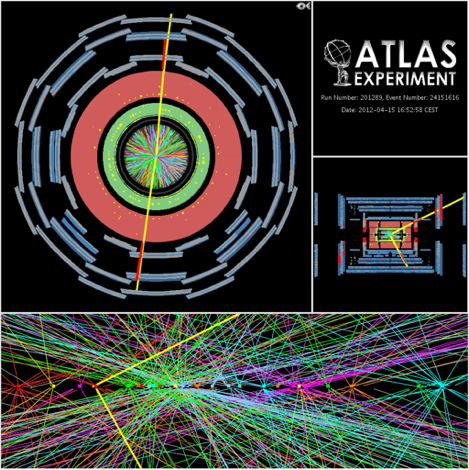
\includegraphics[width=0.6\textwidth]{figures/Zjets_EventDisplay}
  \caption{An event display of a $\ZDY$ + jets event illustrating the effect of pileup interactions}
  \label{fig:Zjetseventdisplay}
\end{figure}

Figure~\ref{fig:METResolution} shows the RMS of the $\MET$ distribution in $Z\TO\mu\mu$ events (where there are no real neutrinos) as a function of the number of the average number of interactions. Under 2011 LHC conditions, this RMS was approximately 9 \GeV, while under 2012 running conditions the resolution worsened to 12 \GeV. This worsening dilutes the efficacy of a cut on $\MET$ to reduce the $\ZDY$ background. 

\begin{figure}[h!]
  %\vspace{20pt}
  \centering
  \captionsetup{justification=centering}

  %\hspace*{-32pt}
  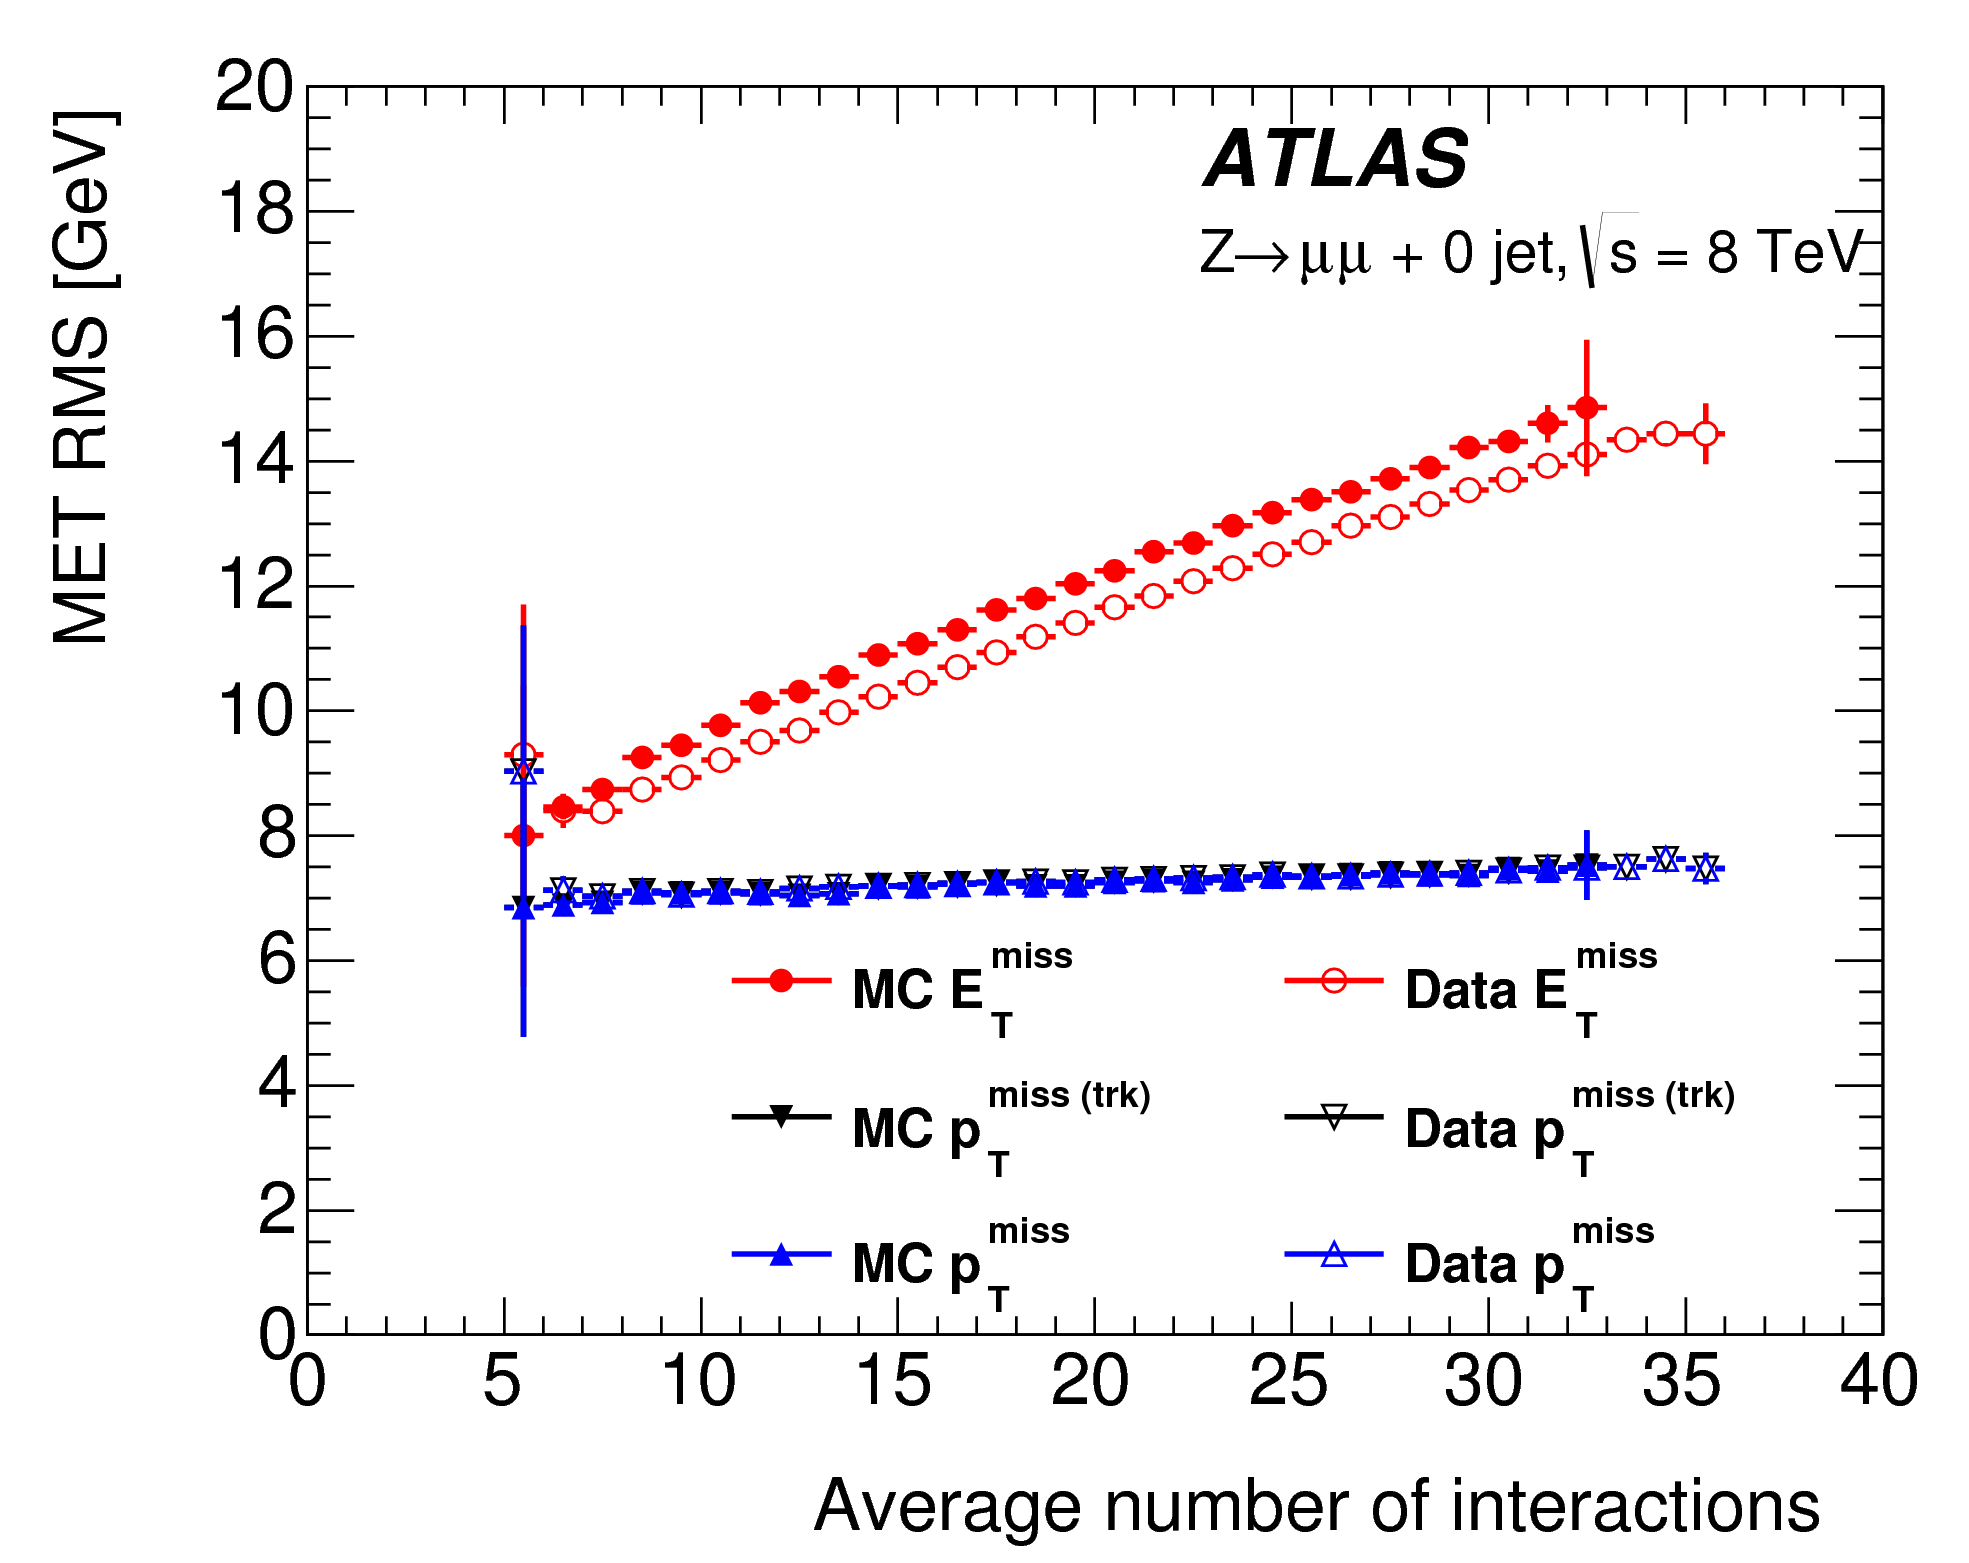
\includegraphics[width=0.6\textwidth]{figures/METResolution}
  \caption{The RMS of different missing transverse momentum definitions as a function of the average number of interactions per bunch crossing}
  \label{fig:METResolution}
\end{figure}

\subsection{Track-based definitions of missing transverse momentum}

Because the increasing number of secondary proton-proton interactions degrades calorimeter-based $\MET$ resolution, a new variable using only contributions from the primary interaction vertex is necessary to further reduce the $\ZDY$ background. While it is not possible to associate calorimeter energy deposits with a particular vertex, individual charged particle tracks in the Inner Detector are associated to unique vertices. Thus, two track-based definitions of \met, using only tracks coming from the primary vertex in the event, are used in the analysis. The simplest variable, $\MPT$, is the vectorial sum of the $\pt$ of all of the tracks in the event and the selected leptons (excluding the tracks associated with the selected leptons to avoid double counting). This is defined in equation~\ref{eqn:MPT}.

\begin{equation}
\vMPT = -\raisebox{-3.0pt}{\bigg(}%
     \displaystyle
     \sum_{\substack{\rm selected \\ \rm leptons}}\,\vpT
   + \sum_{\substack{\rm other \\ \rm tracks}}\,\vpT
   \raisebox{-3.0pt}{\bigg)},
\label{eqn:MPT}
\end{equation} 

In events with hard jets, a better resolution on the \met is obtained by including the calorimeter based measurement of the hard jets rather than the track based measurements. Thus, another variable, $\MPTj$, is defined, using the nominal measurements of $\pT$ for the selected leptons and jets and using tracks rather than calorimeter clusters for the soft component of the \met. This is defined in equation~\ref{eqn:MPTj}.

\begin{equation}
\vMPTj = -\raisebox{-3.0pt}{\bigg(}%
     \displaystyle
     \sum_{\substack{\rm selected \\ \rm leptons}}\,\vpT
   + \sum_{\substack{\rm selected \\ \rm jets}}\,\vpT
   + \sum_{\substack{\rm other \\ \rm tracks}}\,\vpT
   \raisebox{-3.0pt}{\bigg)},
\label{eqn:MPTj}
\end{equation} 

Figure~\ref{fig:METResolution} illustrates that these two new variables accomplish their intended purpose. The resolution as a function of mean number of interactions for both $\MPT$ and $\MPTj$ is much flatter compared to the dependence for $\MET$. 

\begin{figure}[h!]
  %\vspace{20pt}
  \centering
  \captionsetup{justification=centering}

  %\hspace*{-32pt}
  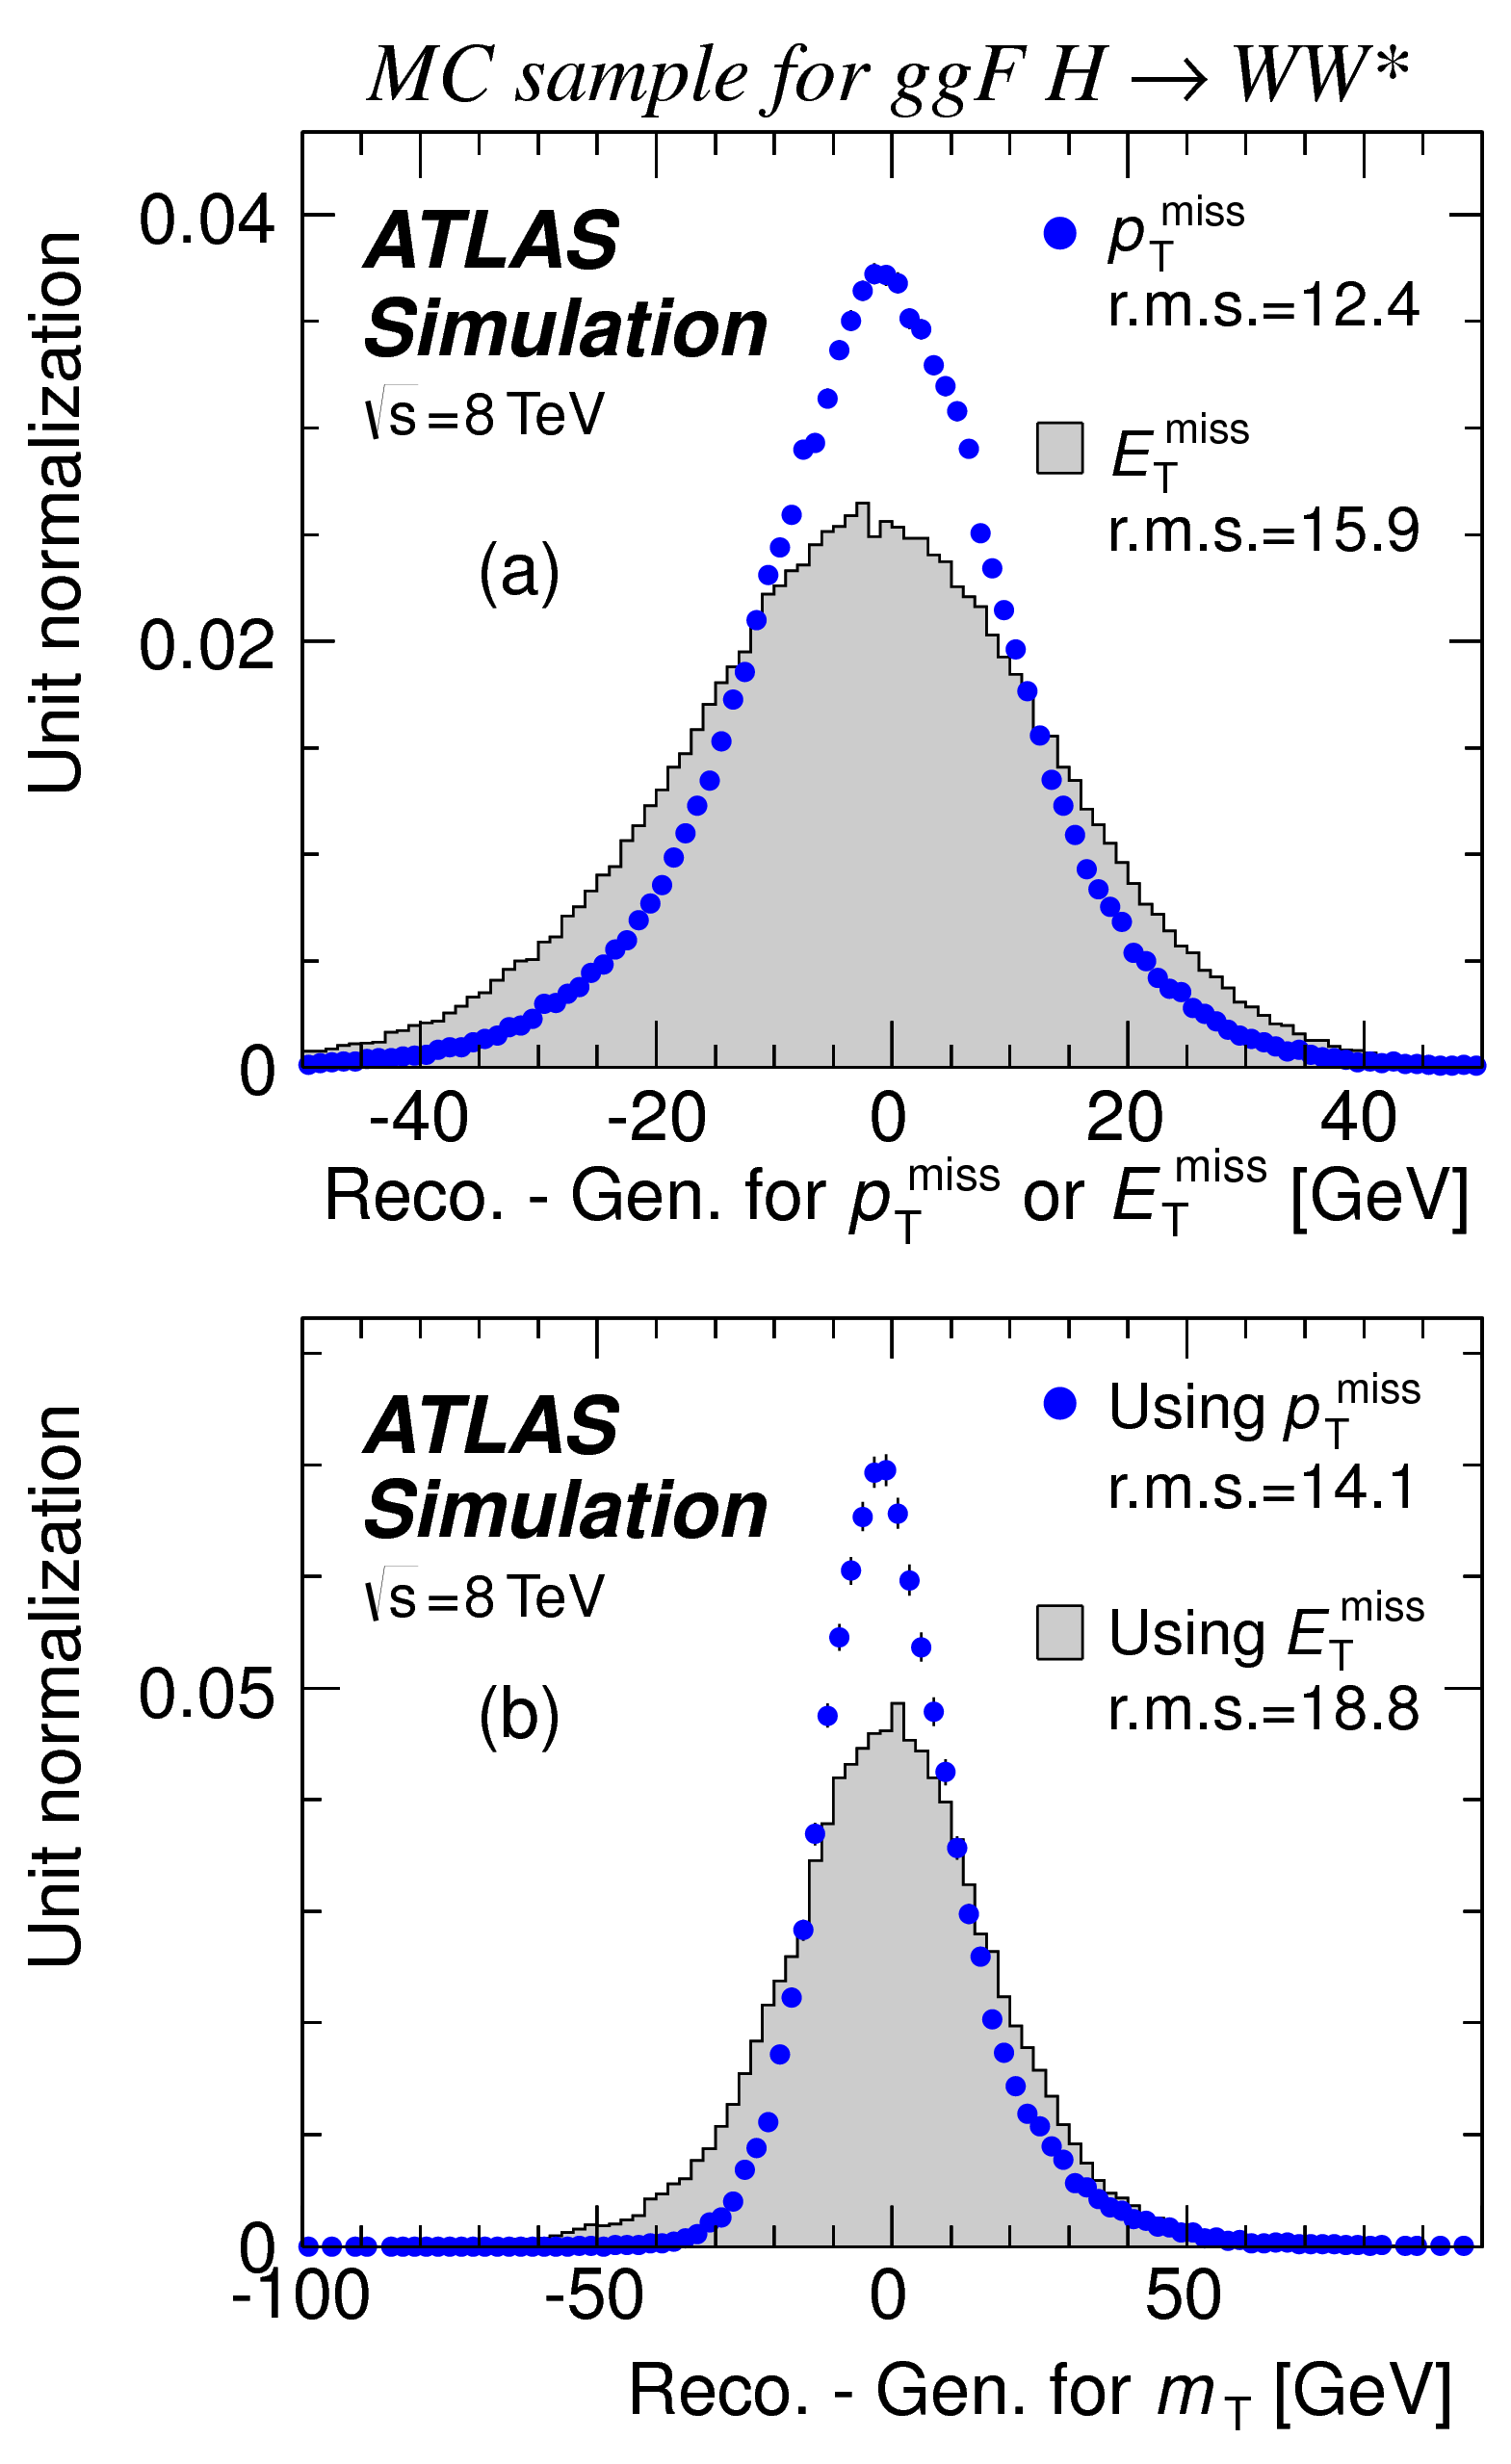
\includegraphics[width=0.6\textwidth]{figures/METResolution2}
  \caption{The difference between the true and reconstructed values of the \met (a) and $\mT$ (b) in a gluon fusion signal sample}
  \label{fig:METResolution2}
\end{figure}

Figure~\ref{fig:METResolution2}a shows the difference between the true and reconstructed values of \met using both the track-based $\MPTj$ and calorimeter based $\MET$. The RMS of the distribution improves by 3.5 \GeV when using $\MPTj$.

\subsection{Distinguishing $\ZDY$ +jets and $\HWW$ topologies}

The track-based definitions of \met were constructed to mitigate degrading performance as a function of pileup. However, an additional variable can be constructed to exploit kinematic and topological differences between the $\ZDY$ background and $\HWW$ signal. Because there are no real neutrinos in the final state (in the case of $Z/\gamma^{*} \TO ee,\mu\mu$ decays), the dilepton system of a $\ZDY$ will be balanced with the jets produced in the hard scatter. A new variable, $\frecoil$, is constructed to estimate the balance between the dilepton system and the jets in the quadrant opposite the dilepton vector in the transverse plane. It is defined in equation~\ref{eqn:frecoil}. The numerator of $\frecoil$ is the magnitude of the vectorial sum of the $\pt$ of jets in the quadrant opposite the dilepton system, weighted by each jet's Jet Vertex Fraction (JVF, described in chapter 2). The denominator is the magnitude of the dilepton $\pt$. 

\begin{equation}
\frecoil = \raisebox{-3pt}{\bigg|} \sum_{{\rm jets\,}j{\rm\,in\,}\wedge}
           \no\jvf_{\,j}\cdot\vpTjet
           ~\raisebox{-3pt}{\bigg|}
           ~\raisebox{-3pt}{\bigg/} \pTll.
\label{eqn:frecoil}
\end{equation}

Figure~\ref{fig:frecoil} shows a shape comparison of the distribution of $\frecoil$ in a simulated $\ZDY$ + jets sample, a $\HWW$ signal sample, and other backgrounds that contain real neutrinos. The $\ZDY$ + jets events tend to be more balanced between the dilepton system and recoiling jets, while the processes containing real neutrinos are less balanced in the transverse plane. Thus, a cut on $\frecoil$ will also reduce the $\ZDY$ + jets background while maintaining a good signal efficiency. 

\begin{figure}[h!]
  %\vspace{20pt}
  \centering
  \captionsetup{justification=centering}

  %\hspace*{-32pt}
  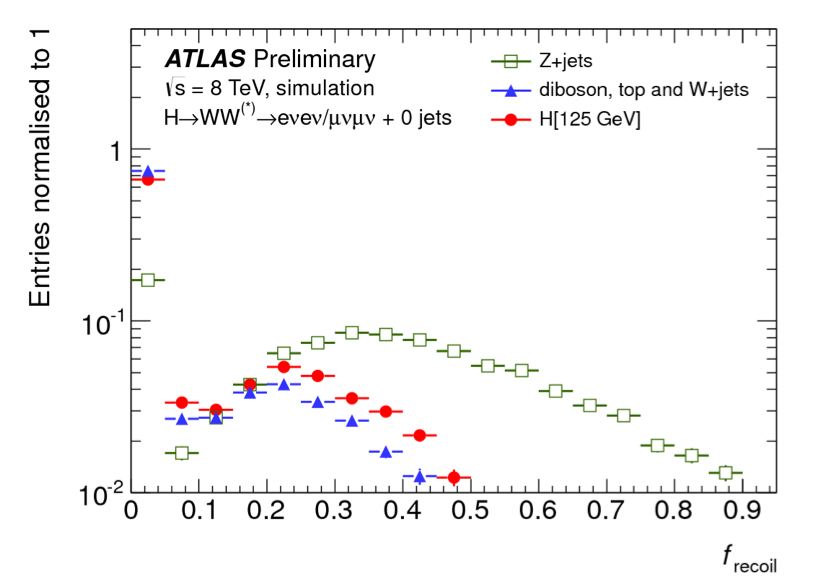
\includegraphics[width=0.6\textwidth]{figures/frecoil}
  \caption{Comparison of $\frecoil$ distributions for $\ZDY$+jets, $\HWW$, and other backgrounds with real neutrinos.}
  \label{fig:frecoil}
\end{figure}

\subsection{Optimizing background reduction cuts}

The cuts on $\MPT$ and $\frecoil$ used to reduce the Z+jets background must be optimized to maximize their efficacy. Figure~\ref{fig:optimization} shows an early attempt to optimize the combination of the two cuts in the gluon fusion zero jet bin. Each bin shows the expected signal significance if the $\MPTrel$ is required to be greater than the left edge of the bin and the $\frecoil$ is required to be less than the top edge of the bin. The figure shows that the best signal significance comes from requiring low values of $\frecoil$ ($< 0.05$) and $\MPTrel$  values greater than 45 GeV. 

\begin{figure}[h!]
  %\vspace{20pt}
  \centering
  \captionsetup{justification=centering}

  %\hspace*{-32pt}
  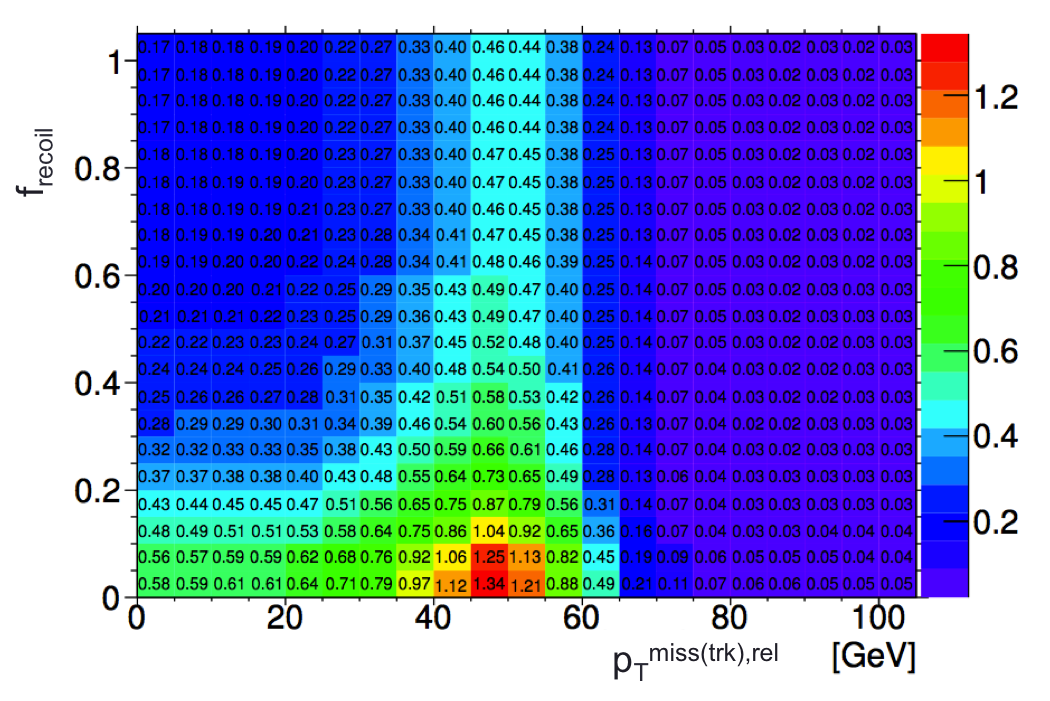
\includegraphics[width=0.8\textwidth]{figures/SFoptimization}
  \caption{Signal significance as a function of cut value in the ggF $\HWW$ with $\Njet = 0$}
  \label{fig:optimization}
\end{figure}


\section{Parameters of interest and statistical treatment}
vents 
As with any search or measurement, there are particular parameters of the Higgs that the $\HWW$ analysis is interested in measuring. In this case, the parameters of interest are the mass of the Higgs boson and its production cross section. Because the \HWWfull process does not have a closed final state, it is not possible to measure the full invariant mass of the particle that may have produced the final state. However, a proxy for the invariant mass using transverse plane information can be defined. This is described in more detail in section~\ref{sec:mt}. The second parameter of interest is the ratio of the measured cross section to that expected from the Standard Model Higgs, which is denoted a $\mu$. This is defined in equation~\ref{eqn:mu}.

\begin{equation}
\mu = \frac{\sigma}{\sigma_{\rm SM}}
\label{eqn:mu}
\end{equation}

All of the likelihoods used in the statistical analysis of the final signal region events are paramaterized as a function of $\mu$. $\mu$ is a natural variable for hypothesis testing, as $\mu = 0$ corresponds to a background only hypothesis and $\mu = 1$ corresponds exactly to a Standard Model Higgs. 

\subsection{Transverse mass}
\label{sec:mt}
Because the longitudinal information about the neutrinos is not attainable, the \HWWfull analysis uses a mass variable, the transverse mass, that exploits information in the transverse plane as a proxy for the full invariant mass. The transverse mass is defined in equation~\ref{eqn:mt}.

\begin{equation}
  \mTH = \sqrt{\left(\eTll + \MPTj\right)^2 - \left|\,\vpTll + \vMPTj\,\right|^2},
\label{eqn:mt}
\end{equation}

Here the $\eTll$ and $\pTll$ are the transverse energy and momentum of the dilepton system, while $\MPTj$ is a proxy for the transverse momentum of the di-neutrino system. The track-based $\MPTj$ is used in the $\mTH$ rather than the calorimeter based $\MET$ because it has a better resolution on the true transverse mass. Figure~\ref{fig:METResolution2}b shows the improvement in the RMS of the difference between the true and reconstructed transverse mass in a ggF signal sample. The RMS improves by 4.7 \GeV using $\MPTj$ in the $\mTH$ calculation.

\subsection[title]{Statistical treatment\footnote{Many thanks to Aaron Armbruster, whose thesis\cite{ArmbrusterThesis} inspired parts of this section.}} 

The statistical analysis of final event candidates is framed as a hypothesis test, where the null hypothesis is background-only (no Standard Model Higgs). The first step in the analysis is to form a likelihood function for the data. In its simplest form, this likelihood is the probability of observing the number of events seen in the final signal region given knowledge of the signal strength. Because observation of events is fundamentally a Poisson counting experiment, this simple likelihood can be expressed as a Poisson probability of observing $N$ events given a total number of predicted signal and background events. This basic likelihood is shown in equation~\ref{eqn:simplepoisson}.

\begin{equation}
\likelihood(\mu) = P\left(N | \mu S + B\right)
\label{eqn:simplepoisson}
\end{equation}

Here, $P$ is the Poisson probability density function, $N$ is the total number of observed events, $\mu$ is the signal strength, $S$ is the predicted number of signal events, and $B$ is the predicted number of background events. 

In particle physics, certain background estimates are commonly normalized in so-called ``control" regions and those predictions are scaled by the same normalization factor in the signal region. This leads to a slightly more complicated likelihood, which is a function of both the signal strength and the background normalization. This is shown in equation~\ref{eqn:mediumpoisson}.

\begin{equation}
\likelihood(\mu, \theta) = P\left(N | \mu S + \theta B\right)P\left(N_{\rm CR} | \theta B_{\rm CR}\right)
\label{eqn:mediumpoisson}
\end{equation}

Here, $\theta$ is a so-called ``nuisance parameter", a parameter that is not a primary parameter of interest but still enters the likelihood. The second Poisson term adds an extra term to the likelihood, enforcing the fact that the background normalization must be consistent with the number of observed events in data in the control region, $N_{\rm CR}$.

So far, these two formulations of likelihoods have assumed a single signal region and do not take into account any shape information of potential discriminating variables. Also, no systematic uncertainties are included in the current likelihood. As mentioned in section~\ref{sec:mt}, the transverse mass is used as the primary discriminating variable in many of the $\HWW$ sub-analyses. Therefore, 
